\section{Baseline Leak Detection Architecture}\label{sec:baseline}

\begin{figure}[t]
	\centering
	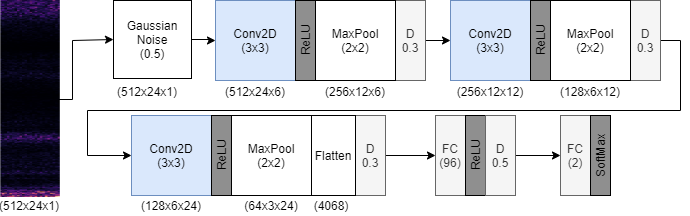
\includegraphics[width=0.95\columnwidth]{images/cnn_flow.png}
	\caption{Baseline CNN architecture for leak detection.}
	\label{fig:cnn}
\end{figure}

We provide a baseline convolutional neural network (CNN) for evaluating the effectiveness of the proposed data driven approach. As input to the CNN, we use a two-dimensional time-frequency representation of the data. This is done by obtaining spectrogram representations of the raw audio by transforming the data from the time-domain using the short time Fourier transform (STFT) with sliding windows over the raw signal. We calculate the magnitude of the STFT with 512 frequency bins for windows of 1024 audio samples with an overlap of 50\%. To create an input patch, 24 spectral frames are concatenated to create patches with a duration of 180 milliseconds seconds, affording near real-time detection. Zero mean and unit variance normalization is applied per frequency bin, using mean and variance parameters calculated from the training data.

The CNN's feature representation network is composed of a Gaussian noise layer on the input, followed by three convolutional layers with max-pooling, and dropout applied at each layer. All layers use Rectified Linear Unit (ReLU) activation. The output is flattened to feed into a dense classification network, which is composed of a single hidden dense layer using ReLU activation which feeds into the final output layer with a SoftMax activation. The full architecture details and hyperparameters are shown in Figure \ref{fig:cnn}.

\section{Experimental Design}\label{sec:exps}

To investigate the effectiveness of a deep learning approach for compressed air leak detection, we perform a variety of experiments using the baseline CNN described in Section \ref{sec:baseline}. In addition to establishing baseline results for further research, we perform experiments designed to evaluate the importance of recording conditions for training, such as background noise and microphone placement.

In the first experiment, \textit{E1}, we evaluate the CNN architecture on each of the described recording conditions using microphone 1, which was closest to the leak. We employ a leave-one-out cross validation (\textit{LOO}) approach, in which we train using two of the recording sessions and test with the left out recording session. This is done for three folds so each session is held out once. The results are averaged over the three splits. This validation scheme ensures that there is no data leak between the training and testing datasets as well as helps to detect overfitting in a specific session.

Experiment \textit{E2} evaluates the ability to detect air leaks in noisy conditions when the model is trained from data with minimal background noise, as in the case of lab noise. The detection models are trained using data with lab noise from all three sessions of a specific leak state. The models are then evaluated using all three sessions of a leak state containing a specified noise type, either workshop or hydraulic. The results are averaged over the three sessions.

In some cases, noise conditions vary between recording locations, so leak detection conditions may have different background noise than the originally trained model. To evaluate detection performance under this scenario in experiment \textit{E3} models are trained using data containing one type of background noise, and evaluated on test data with the other type. For example, models trained using data with hydraulic background noise are evaluated using data with workshop background noise. 

In cases where no realisitic background noise can be obtained for the training process, data augmentation \cite{zhong2017randomerase, Zhang2018:mixup, Park2019:spec_aug} might be a possible approach to regularize the input data. For this experiment, \textit{E4}, we combine three common spectral augmentation techniques: random erasing \cite{zhong2017randomerase}, SpecAugment \cite{Park2019:spec_aug}, and Mixup \cite{Zhang2018:mixup}. Each of these augmentation methods are selected to be applied to an input spectrogram with 50\% probability and in a random order. The model is then trained by augmenting the data with no background noise using the above methods. Both the original data, and the augmented data are included during data, doubling the size of the training dataset.

The final experiment, \textit{E5}, is to evaluate the effect of the microphone positioning on classification performance. In this experiment, LOO cross validation is performed for all conditions for each microphone. This is intended to provide first insights into where best to place a microphone in an air leak detection system.

\section{Results}\label{sec:res}

\begin{table}[h]
    \centering
    \caption{Classification accuracy (\%) on noisy test data for various training schemes. \textbf{CNN LOO} show the classification results for the CNN for leave-one-out cross validation. \textbf{OtherNoise} shows the results on the noisy test data when training using data with the other type noise. \textbf{NoNoise} shows the results on the test data when training on data with no background noise. \textbf{AUG} shows the results when training with data with no noise but using data augmentation techniques. (The * indicates data is missing due to corruption as discussed in Section \ref{sec:dataset}.)}
    \begin{tabular}{l l c c c c c}
    \toprule
    Condition & Noise Type & CNN LOO (\textit{E1}) & NoNoise (\textit{E2}) & OtherNoise (\textit{E3}) & AUG (\textit{E4}) \\ \midrule
    
    Vent Leak & Lab & $96.63\pm3.07$ & - & - & - \\
    Vent Low  & Lab & $94.45\pm5.88$ & - & - & -  \\ 
    Tube Leak & Lab & $99.11\pm0.77$ & - & - & -  \\ \midrule
    Average   & Lab & $96.73\pm3.90$ & - & - & -  \\ \midrule
    
    Vent Leak & Work Low* & $92.65\pm3.73$ & $68.42\pm13.0$ & $98.01\pm1.02$ & $89.52\pm1.28$ \\
    Vent Low  & Work Low  & $91.17\pm0.77$ & $75.21\pm8.80$ & $87.22\pm9.02$ & $79.84\pm5.70$ \\
    Tube Leak & Work Low  & $97.43\pm1.47$ & $59.81\pm24.0$ & $94.35\pm6.32$ & $81.43\pm9.49$ \\ \midrule
    Average   & Work Low  & $93.89\pm3.43$ & $67.81\pm15.3$ & $93.19\pm5.45$ & $83.60\pm5.49$ \\ \midrule
    
    Vent Leak & Work & $98.46\pm0.88$ & $58.82\pm19.8$ & $96.98\pm2.30$ & $83.38\pm5.44$ \\
    Vent Low  & Work & $93.35\pm4.96$ & $64.75\pm9.98$ & $89.57\pm9.51$ & $78.51\pm9.82$ \\
    Tube Leak & Work & $97.02\pm2.73$ & $54.67\pm19.9$ & $95.12\pm4.00$ & $71.24\pm6.29$ \\ \midrule
    Average   & Work & $96.28\pm3.66$ & $59.41\pm16.5$ & $93.89\pm5.27$ & $77.71\pm7.18$ \\ \midrule
    
    Vent Leak & Hydr Low & $98.55\pm1.29$ & $33.49\pm0.45$ & $95.93\pm4.72$ & $80.34\pm7.88$ \\
    Vent Low  & Hydr Low & $87.62\pm6.58$ & $58.56\pm13.4$ & $87.38\pm6.28$ & $67.92\pm18.8$ \\
    Tube Leak & Hydr Low & $96.03\pm3.73$ & $55.27\pm20.2$ & $94.67\pm3.70$ & $62.98\pm20.3$ \\ \midrule
    Average   & Hydr Low & $94.07\pm6.27$ & $49.11\pm11.4$ & $92.66\pm4.90$ & $70.41\pm15.7$ \\ \midrule
    
    Vent Leak & Hydr & $94.24\pm2.13$ & $38.55\pm6.69$ & $90.54\pm2.79$ & $71.84\pm9.46$ \\
    Vent Low  & Hydr & $92.75\pm2.77$ & $58.33\pm14.3$ & $92.25\pm2.36$ & $67.33\pm4.99$ \\ 
    Tube Leak & Hydr & $98.39\pm0.81$ & $41.46\pm14.6$ & $94.26\pm2.85$ & $54.72\pm13.8$ \\\midrule
    Average   & Hydr & $95.24\pm3.20$ & $46.11\pm11.9$ & $92.35\pm2.67$ & $64.64\pm9.41$ \\
    
    \bottomrule
    \end{tabular}
	\label{tab:noise-train}
\end{table}

The results for experiments \textit{E1} to \textit{E4} are presented in Table \ref{tab:noise-train}. \textit{E1} results show that a data driven approach using CNNs has the potential for air leak detection, even in noisy conditions. 
When training with the same type of background noise contained in the evaluation data, we see results similar to the no noise condition. 
Indicating that background noise has minimal effect on the classification performance when models are trained with the same type of noise in the evaluation data. Background noise characteristics, however, may not be consistent over time, and therefore, methods to account for varying background noise should be evaluated. Additionally, the vent leak under low pressure conditions (\textit{vent low}) is consistently harder to detect, presumably because the lower pressure results in lower turbulence so the leak is not as loud.

In \textit{E2}, the performance on noisy data when training with clean data is evaluated. In this, case classification performance severely degrades compared to \textit{E1}. Alternatively, in \textit{E3} we see only a minor decrease in performance across all conditions when training with data that contains a different type of background noise than the evaluation data. One possible explanation may be that the network is overfitting to frequencies patterns that are masked by the newly introduced noise, while training with noisy data requires the the network to identify harder to find patterns resulting in a more stable model \footnote{In the case of vent leak with low hydraulic noise, the other noise data, the vent leak and workshop low, is the dataset with a missing session recording. To account for this, we substituted the missing session data with the corresponding session data from vent leak workshop data.}. Training with data augmentation performed on the no noise data, in \textit{E4}, results in significantly better performance than training with no noise alone. However, it is not a substitute for training with data already containing background noise. 

\begin{table}[H]
    \centering
    \caption{\textit{E5}, classification accuracy (\%) of LOO cross validation for different microphone configurations using a CNN classification model.}
    \begin{tabular}{l l l c c c}
    \toprule
    Condition & Noise Type & MIC 1 & MIC 2 & MIC 3 & MIC 4 \\ \midrule
    
    Vent Leak & Lab & $96.63\pm3.07$ & $94.37\pm4.61$ & $99.58\pm0.36$ & $93.81\pm5.22$\\
    Vent Low  & Lab & $94.45\pm5.88$ & $88.34\pm9.30$ & $87.20\pm15.2$ & $93.64\pm5.68$\\ 
    Tube Leak & Lab & $99.11\pm0.77$ & $92.65\pm3.69$ & $99.00\pm0.84$ & $93.31\pm5.36$\\ \midrule
    Average   & Lab & $96.73\pm3.90$ & $91.78\pm6.13$ & $95.25\pm9.73$ & $93.59\pm4.70$ \\ \midrule
    
    Vent Leak & Work & $98.46\pm0.88$ & $71.78\pm28.3$ & $96.89\pm4.21$ & $93.67\pm4.35$ \\
    Vent Low  & Work & $93.35\pm4.96$ & $92.92\pm5.06$ & $92.83\pm5.49$ & $92.03\pm5.02$\\ 
    Tube Leak & Work & $97.02\pm2.73$ & $64.79\pm33.3$ & $92.98\pm1.23$ & $86.88\pm4.35$ \\ \midrule
    Average   & Work & $96.23\pm3.66$ & $76.50\pm25.4$ & $94.24\pm4.03$ & $90.86\pm5.02$ \\ \midrule
    
    Vent Leak & Hydr & $94.24\pm2.13$ & $91.67\pm0.28$ & $93.14\pm0.82$ & $91.08\pm0.59$ \\
    Vent Low  & Hydr & $92.75\pm2.77$ & $92.13\pm1.85$ & $92.95\pm3.33$ & $91.56\pm1.76$\\ 
    Tube Leak & Hydr & $98.39\pm0.81$ & $71.33\pm33.2$ & $98.48\pm0.38$ & $91.52\pm2.85$\\ \midrule
    Average   & Hydr & $95.24\pm3.20$ & $85.05\pm19.6$ & $94.86\pm3.22$ & $91.39\pm1.71$\\ 
    
\bottomrule
    \end{tabular}
	\label{tab:mic-logo}
\end{table}

In the final experiment, \textit{E5}, the effect of microphone placement on classification performance is evaluated, and the results are presented in Table \ref{tab:mic-logo}. Microphone 1 has the best average results over all three noise conditions. This was expected as it was the closest microphone and oriented at an angle that the air would not blow directly on the microphone. Microphone 3 has similar results indicating that the angle and direct air contact on the microphone may only have limited effect on performance. Microphone 2, being further away but oriented towards the leak, has the least consistent and lowest performance. Interestingly, microphone 4 shows only a minor degradation in performance, even though it was located the furthest away from the leak source, located near the ceiling, and not oriented toward the source. One possible reason might be the reflections of the leak sound that are captured with the omnidirectional microphone from several sides.